\begin{multicols}{2}
 This fully open-source sensor is a time-of-flight based distance sensor based on two VL53L0X from STMicroelectronics. It is aimed at providing accurate distance measurements at a high sampling rate which can go up to 50Hz. It is also largely configurable and offers an external interrupt functionality. It accepts a wide input voltage range and will adapt the \iic voltages to the input power.
 \columnbreak
 \subsection{Features}
 \begin{itemize}
  \item Fully open-source. Adapt it to your needs
  \item Input voltage from 3.0V to 5.5V
  \item Low power consumption
  \item Distance sensing from 0 to 200 cm
  \item \iic communication bus
  \item External interrupts functionality
  \item Calibration routines
  \item Programmable \iic address
  \item DIP switches for boot configuration
 \end{itemize}
\end{multicols}

\subsection{Typical application}

\begin{figure}[h]
 \centering
 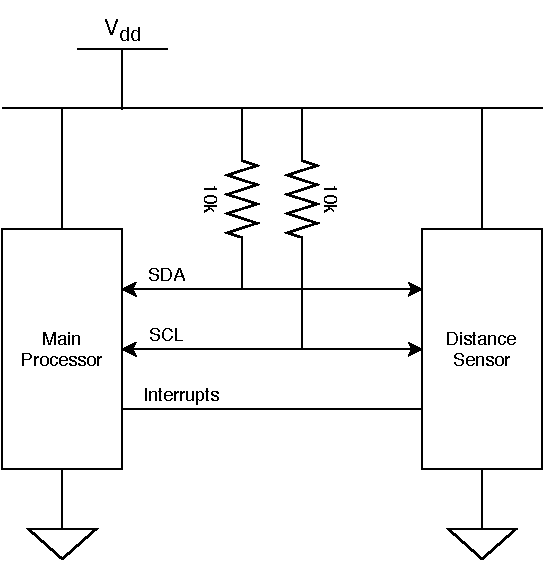
\includegraphics[width=0.5\textwidth]{../img/dual-vl53l0x-sensor.pdf}
\end{figure}